\documentclass[11pt,a4paper]{article}
\usepackage{a4wide,url,graphicx}
\usepackage[utf8]{inputenc}
\usepackage[russian]{babel}
\usepackage{tikz}
\usetikzlibrary{shapes.misc}
\usetikzlibrary{arrows.meta}

\parskip3pt
\parindent0pt

\title{Different Versions of the Laws of\\ Technical Evolution within TRIZ}

\author{Compiled by Hans-Gert Gräbe, Leipzig}

\date{Version of 07 December 2019}

\begin{document}
\maketitle

I started a discussion on that topic at
Facebook\footnote{\url{https://www.facebook.com/groups/111602085556371}}.
Since this discussion is in Russian and German, this compilation is also in
these languages. Only the headings are in English.

\section*{The version as presented in the improved TDS material}

The following diagram was compiled using the \texttt{tikz} \LaTeX-package from
the corresponding (improved) diagram in the Exercises of the TRIZ Summit
Cup\footnote{\url{https://triz-summit.ru/contest/cup-tds-2019-2020/contest-2019-2020/}}.

\begin{center}
\newcommand{\law}[2]{\parbox{#1cm}{\small\centering #2}}
\tikz[>={Triangle[length=3pt 9, width=3pt 3]}] {
  
\node[draw] at (5,7) [rectangle]
(A1) {\law{3}{Закон повышения идеальности}};

\node[draw] at (0,6) [rectangle]
(A2) {\law{4}{Закон повышения полноты частей системы (Закон полноты выполнения принципа действия)}};

\node[draw] at (0,2) [rectangle]
(A3) {\law{4}{Закон повышения согласованности частей системы}};

\node[draw] at (0,4) [rectangle]
(A4) {\law{4}{Закон проводимости: энергии, потоков и др.}};

\node[draw] at (5,5) [rectangle]
(A5) {\law{3}{Закон неравномерного развития частей системы}};

\node[draw] at (10,0) [rectangle]
(A6) {\law{4}{Тенденция развития ТС по S-образной кривой}};

\node[draw] at (0,0) [rectangle]
(A7) {\law{4}{Тенденция вытеснения человека из ТС}};

\node[draw] at (10,4) [rectangle]
(A8) {\law{4}{Закон повышения управляемости / вепольности}};

\node[draw] at (5,1) [rectangle]
(A9) {\law{3}{Закон повышения динамичности}};

\node[draw] at (5,3) [rectangle]
(A10) {\law{3}{Закон перехода в надсистему}};

\node[draw] at (10,6) [rectangle]
(A11) {\law{4}{Закон перехода с макроуровня на микроуровень}};

\node[draw] at (10,2) [rectangle]
(A12) {\law{4}{Тенденция развития за счет свертывания или развертывания ТС}};

\draw[->] (A1) -- (2.8,7) |- (A2) ;
\draw[->] (2.8,7) |- (A3);
\draw[->] (2.8,7) |- (A4);
\draw[->] (2.8,7) |- (A5);
\draw[->] (2.8,7) |- (A7);
\draw[->] (2.8,7) |- (A9);
\draw[->] (2.8,7) |- (A10);
\draw[->] (A2) -- (-2.7,6) |- (A7);
\draw[->] (A5) -- (7.2,5) |- (A9);
\draw[->] (7.2,5) |- (A10);
\draw[->] (7.2,5) |- (A6);
\draw[->] (A1) -- (7.5,7) |- (A8) ;
\draw[->] (7.5,7) |- (A11) ;
\draw[->] (7.5,7) |- (A12) ;
\draw[->] (A8) -- (12.5,4) |- (A12) ;
}
\end{center}

\section*{The Laws as given in the first version of the TDS material}

\begin{center}
  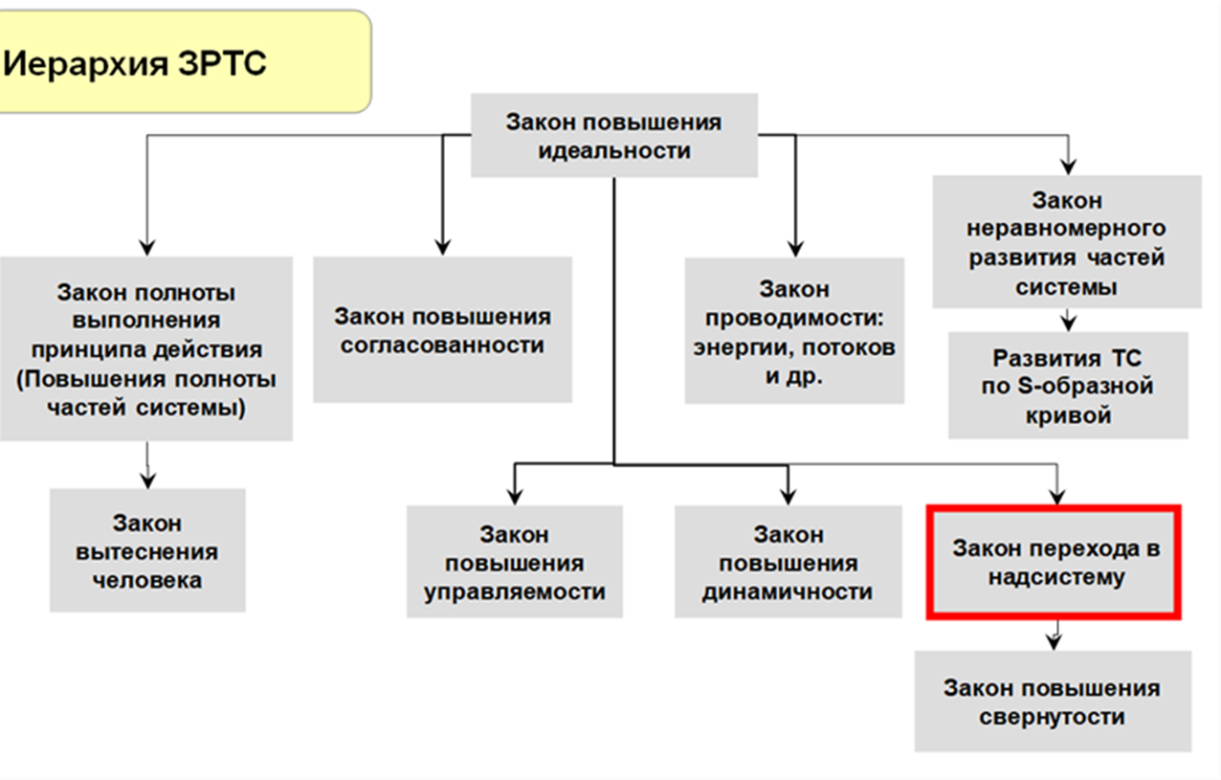
\includegraphics[width=.9\textwidth]{oE4yUs.png}
\end{center}

\section*{Laws as explained in (Koltze/Souchkov, ch. 4.8)}

(Koltze/Souchkov)\footnote{ Karl Koltze, Valeri Souchkov. Systematische
  Innovation. ISBN 978-3-446-45127-8.} различают законы на одной стороне и
эволюционные линии и тенденции развития технических систем на другой.

Gesetze der Evolution technischer Systeme
\begin{enumerate}\itemsep0pt
\item Gesetz der Vollständigkeit des Systems
\item Gesetz der Vollständigkeit des Obersystems
\item Gesetz der Erhöhung der Idealität
\item Gesetz der ungleichen Entwicklung von Systemteilen
\item Gesetz der Erhöhung von Stoff-Feld-Interaktionen
\end{enumerate}

Evolutionslinien und -trends technischer Systeme
\begin{enumerate}\itemsep0pt
\item Dynamisierung
\item Koordination und Evolution der Rhythmik
\item Gestalt- und Formkoordination
\item Evolution der Geometrie
\item Erhöhung des Energie-Leitvermögens
\item Übergang auf die Mikroebene
\item Zunehmende Steuerbarkeit
\item Erhöhung der Automation
\item Übergang zum Obersystem
\item Zusammenfall
\end{enumerate}

\subsection*{Russian Translation}

Законы эволюции технических систем
\begin{enumerate} \itemsep0pt
\item Закон полноты системы
\item Закон полноты надсистемы
\item Закон повышения идеальности
\item Закон неравномерного развития частей системы
\item Закон повышения взаимодействия вещества и полей
\end{enumerate}

Линии эволюции и тенденции технических систем
\begin{enumerate} \itemsep0pt
\item Динамизация
\item Координация и эволюция ритма
\item Координация образа и формы
\item Эволюция геометрии
\item Повышение электропроводности
\item Переход на микроуровень
\item Повышение управляемости
\item Увеличение степени автоматизации
\item Переход к надсистеме
\item Совпадение 
\end{enumerate}

\section*{German Wikipedia}

\textbf{Begriffsklärung:} Neben dem Originalbegriff Gesetze der Entwicklung
von Systemen (Alt\-schuller, S. 186) [3] werden auch Definitionen wie
Technische Entwicklungstrends [15], Gesetz\-mäßigkeiten der technischen
Evolution [9] oder Evolutionsprinzipien technischer Systeme [14] verwendet. Im
englischen Sprachgebrauch verwendet man für dieses Tool die folgenden
Be\-zeichnungen: Trends of Evolution [16], Trends of Technological Evolution
[17], Patterns of Evolution [18] oder TESE – Trends of Engineering System
Evolution [6].

\textbf{Beschreibung:} Die Gesetze der Entwicklung von Systemen geben
Hinweise, wie sich ein technisches System entwickeln wird. Dabei stützt man
sich auf die Beobachtungen in der Historie und kann somit gewisse Voraussagen
treffen. Diese Voraussagen sind sehr abstrakt und stellen eher eine
Aufgabenstellung oder eine Vision dar, die es ermöglicht, Ideen für konkrete
weitere Schritte zu entwickeln.

In der Literatur finden sich momentan nur die 8 Gesetze, die Altschuller
selbst aufgestellt hat oder die acht von Terninko, Zusman und Zlotin. Es gibt
aber umfangreiche weitere Arbeiten zu diesen Entwicklungsgesetzen, die ein
wesentlich verbessertes Arbeiten zulassen. Im Folgenden werden die 8 Gesetze
genannt, wie sie von Altschuller[3] beschrieben wurden:
\begin{enumerate}
\item \textbf{Gesetz der Vollständigkeit der Teile eines Systems:} Notwendige
  Bedingungen für die Lebensfähigkeit eines technischen Systems ist das
  Vorliegen der Hauptteile des Systems und eine minimale Funktionsfähigkeit
  derselben.
\item \textbf{Gesetz der „energetischen Leitfähigkeit“ eines Systems:} Eine
  notwendige Bedin\-gung für die Lebensfähigkeit eines technischen Systems ist
  der Energiefluss durch alle Teile des Systems.
\item \textbf{Gesetz der Abstimmung der Rhythmik der Teile eines Systems:}
  Eine notwen\-dige Bedingung für die Lebensfähigkeit eines technischen
  Systems ist die Abstimmung der Rhythmik (der Schwingungsfrequenz, der
  Periodizität) aller Teile des Systems.
\item \textbf{Gesetz der Erhöhung des Grades der Idealität eines Systems:} Die
  Entwicklung aller Systeme verläuft in Richtung auf die Erhöhung des Grades
  der Idealität.
\item \textbf{Gesetz der Ungleichmäßigkeit der Entwicklung der Teile eines
  Systems:} Die Entwicklung der Teile eines Systems verläuft ungleichmäßig; je
  komplizierter das System ist, umso ungleichmäßiger verläuft die Entwicklung
  seiner Teile.
\item \textbf{Gesetz des Übergangs in ein Obersystem:} Nach Erschöpfung seiner
  Entwicklungs\-möglichkeiten wird ein System als ein Teil in ein Obersystem
  aufgenommen: Dabei erfolgt die weitere Entwicklung auf der Ebene des
  Obersystems.
\item \textbf{Gesetz des Übergangs von der Makroebene zur Mikroebene:} Die
  Entwicklung der Arbeitorgane eines Systems erfolgt zunächst auf der
  Makroebene und anschließend auf der Mikroebene.
\item \textbf{Gesetz der Erhöhung des Anteils von Stoff-Feld-Systemen:} Die
  Entwicklung technischer Systeme verläuft in Richtung auf die Erhöhung des
  Anteils und der Rolle von Stoff-Feld-Wechselwirkungen.
\end{enumerate}

\subsection*{Russian Translation}

\textbf{Определение терминов:} В дополнение к оригинальной концепции законов
развития систем (Altschuller, p. 186) [3] также существуют такие определения,
как Технические Тенденции Развития [15], Законы Технической Эволюции [9] или
Принципы Эволюции Технических Систем [14]. На английском для этого инструмента
используются следующие обозначения: Тенденции Эволюции [16], Тенденции
Технологической Эволюции [17], Паттерны Эволюция [18] или TESE - Тенденции
Развития Инженерных Систем [6].

\textbf{Описание:} Законы развития систем дают указания о том, как техническая
система будет развиваться. Основываясь на наблюдениях истории системы делаются
определенные прогнозы. Эти предсказания очень абстрактны и скорее представляют
задачу или видение, которое позволяет разработать идеи для конкретных
дальнейших шагов.

На данный момент в литературе всего 8 законов, которые Альтшуллер сам
опубликовал или те из публикации Тернинко, Зусмана и Злотина. Есть обширная
дальнейшая литература по этим законам развития, которые позволяют значительно
улучшить работу. Ниже приведены 8 законов как описано Альтшуллером [3]:
\begin{enumerate}
\item \textbf{Закон полноты частей системы:} Необходимым условием
  жизнеспособности технической системы является наличие основных частей
  системы и минимальная их работоспособность.
\item \textbf{Закон „энергетической проводимости“ системы:} Одно необходимое
  условие жизнеспособности технической системы поток энергии через все его
  части.
\item \textbf{Закон настройки ритма частей системы:} Необходимое условие
  жизнеспособности технической системы настройка ритма (частота колебаний,
  периодичность) всех частей системы.
\item \textbf{Закон повышения степени идеальности системы:} Развитие всех
  систем идет в направлении повышения степени идеальность.
\item \textbf{Закон неравномерности развития частей системы:} Развитие частей
  системы неравномерно; чем сложнее система, тем неравномернее развитие его
  частей.
\item \textbf{Закон перехода в надсистему:} После исчерпания возможностей его
  развития система становится частью надсистемы и дальнейшее развитие
  происходит на уровне надсистемы.
\item \textbf{Закон перехода от макроуровня к микроуровню:} Развитие рабочих
  органов системы происходит в первую очередь на макроуровне, а затем на
  микроуровне.
\item \textbf{Закон увеличения вклада вепольных систем:} Развитие технических
  систем идет в направлении увеличения доля и роли вещественно-полевых
  взаимодействий.
\end{enumerate}

\section*{V.M. Petrov}

A list of the content of chapter 4 „Законы Развития Технических Систем (ЗРТС)“
of Petrov's book „Теория решения изобретательских задач –
ТРИЗ“\footnote{Петров В. М. Теория решения изобретательских задач – ТРИЗ:
  учебник по дисциплине «Алгоритмы решения нестандартных задач». ISBN:
  978-5-91359-207-1. }
\begin{itemize}\itemsep0pt
\item[] 4.1. Общие представления
\item[] 4.2. Закон S–образного развития систем
\item[] 4.2.1. Общие представления
\item[] 4.2.2. Огибающие кривые
\item[] 4.3. Структура законов развития технических систем
\item[] 4.4. Законы организации систем
\item[] 4.4.1. Общие соображения
\item[] 4.4.2. Закон полноты частей системы
\item[] 4.4.3. Закон проводимости потоков
\item[] 4.4.4. Закон минимального согласования частей и параметров системы
\item[] 4.4.5. Построение новой системы
\item[] 4.5. Законы эволюции систем
\item[] 4.5.1. Общие сведения
\item[] 4.5.2. Закон увеличения степени идеальности
\item[] 4.5.3. Закон увеличения степени управляемости
\item[] 4.5.4. Закон увеличения степени динамичности
\item[] 4.5.5. Закон перехода на микроуровень
\item[] 4.5.6. Закон перехода системы в надсистему
\item[] 4.5.7. Закон увеличения степени согласованности
\item[] 4.5.8. Закон свертывания – развертывания ТС
\item[] 4.5.9. Закон сбалансированного развития систем
\item[] 4.6. Законы развития технических систем Г. С. Альтшуллера
\item[] 4.7. Прогнозирование развития технических систем
\item[] 4.7.1. Основные понятия прогнозирования
\item[] 4.7.2. Прогнозирование с использованием ТРИЗ
\item[] 4.7.3. Анализ уровня развития системы
\item[] 4.7.4. Экспресс-прогноз
\end{itemize}
\end{document}
